\documentclass[../main.tex]{subfiles}
\begin{document}
\setchapterstyle{kao}
\setchapterpreamble[u]{\margintoc}
\chapter[Electrodynamics and differential forms]{Electrodynamics and differential forms}
\labch{electrodin-diff-forms}
\section[Reformulation of electrodynamics with differential forms]{Reformulation of (classical) electrodynamics with differential forms}
The first application of this theory is the reformulation of classical electrodynamics in terms of differential forms.
\paragraph{\underline{Setting:}} We will consider a manifold  $\mathbf{M}$ with {\color{red}$\textrm{dim}\mathbf{M}=4$} as space-time. To start with, we will be even more specific, we will consider the \href{https://it.wikipedia.org/wiki/Spaziotempo_di_Minkowski}{Minkowski space}\sidenote{"spaziotempo di Minkowski" in Italian.}$\mathbb{M}$, as known, regarded as a linear space over a manifold that can be identified with $\mathbf{M}\cong\mathbb{M}^4$, which means it is a \underline{\textbf{flat}} manifold. This fact as two important consequences:
\begin{enumerate}
    \item there exist infinitely many global charts and coordinates, we will denote them with $\left(x^0,x^1,x^2,x^3\right)\equiv \left(x^0,\vec{x}\right)$;
    \item there is a natural identification\sidenote{As always happens, if you have a linear space, the tangent to the linear space can be identify with the space itself, even though sometimes is convenient to distinguish them.}
    between the tangent space to the Minkowski at a point and the Minkowski space itself: $T_P\mathbb{M}=\mathbb{M}$.
\end{enumerate}
But the Minkowski space is not just $\mathbb{R}^4$, but is $\mathbb{R}^4$ equipped with:\index{Lorentzian metric}
\[
\textrm{\textbf{Lorentzian metric:} biliniear, symmetric, signature} \ (1,3)
\]
\[
\langle v,w\rangle_{\underset{\mathclap{\tikz \node {$\uparrow$} node [below=1ex] {\footnotesize metric};}}{g}}=\sum\underset{\mathclap{\tikz \node {$\uparrow$} node [below=3ex] {\footnotesize does not depend on $x$};}}{g_{\mu\nu}}v^\mu w^\nu \quad \forall \ v,w \in T_P\mathbb{M}
\]
\begin{marginfigure}
	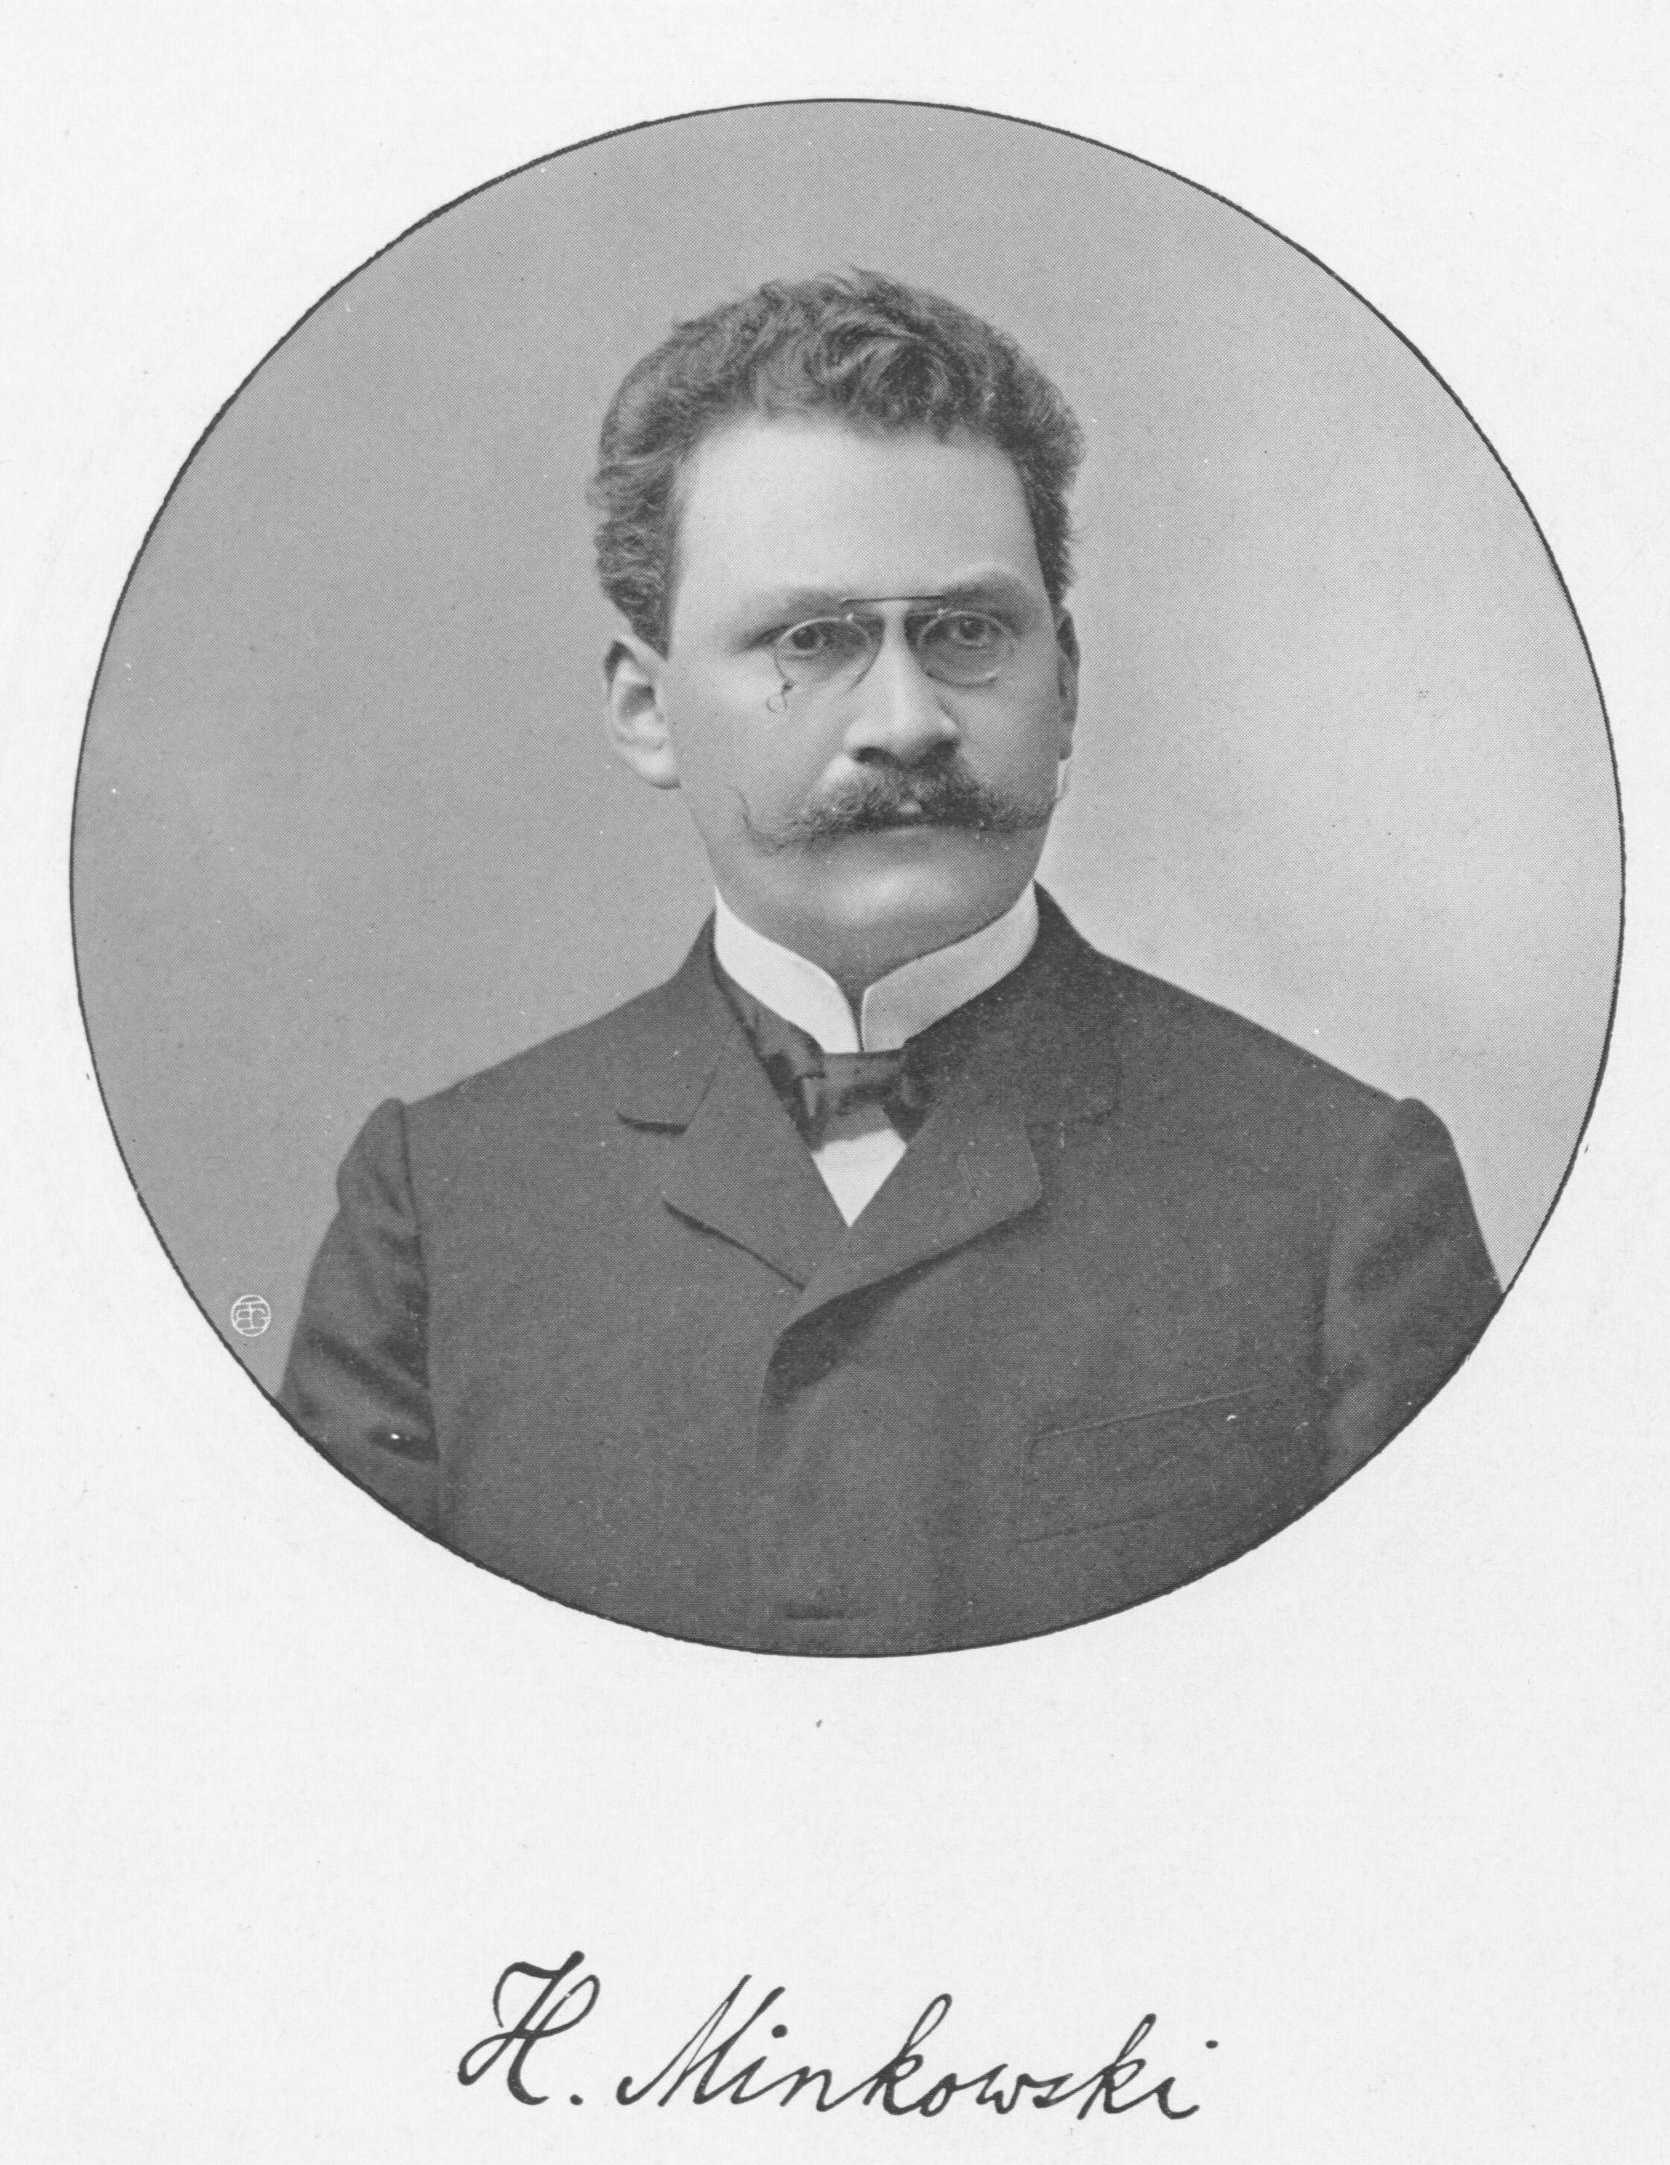
\includegraphics[width=1\linewidth]{images/De_Raum_zeit_Minkowski_Bild.jpg}
	\caption[Photo of Minkowski]{From \href{https://commons.wikimedia.org/wiki/File:De_Raum_zeit_Minkowski_Bild.jpg}{Wikimedia}: Hermann Minkowski (1864-1909) found that the theory of special relativity, introduced by his former student Albert Einstein, could be best understood as a four-dimensional space, since known as the Minkowski spacetime.}
	\labfig{Minkowski}
\end{marginfigure}
The signature can be:
\[
\begin{cases}
    \textrm{Positive signature:}\;(-,+,+,+)=(1,3) \;\; &\textrm{used in General Relativity}\\
    \textrm{Negative signature:}\;(+,-,-,-)=(3,1) &\textrm{used in High Energy Physics}
\end{cases}
\]
according to the convection. The $g$ has subscript to remind our self that it comes from a metric (bilinear and symmetric) and that it is not the inner product of a Hilbert space (sesquilinear and hermitian). As we heard several times, one of the basic principle of the theory is that an inertial frame, in the physical reality, corresponds to an inertial frame in our theory.
\[
\text{\parbox{4 cm}{\centering Inertial \\[-4pt] frame \\[-4pt] (structure)}}\longleftrightarrow\text{\parbox{4 cm}{\centering Lorentzian \\[-4pt] frame  \\[-4pt] (basis/chart)}}
\]
Notice that the word \textit{frame} is used with two different meanings on the two sides of the arrow:
\begin{itemize}
    \item \textbf{Physical reality}: inertial frame is a macroscopic rigid structure with three orthonormal axes and a clock. It is an inertial structure in the laboratory.
    \item \textbf{Mathematical reality}: Lorentian frame is a basis (or system of coordinates) which has the special property that it can diagonlize the metric: in an inertial frame $\leftrightarrow$ Lorential frame if we take the vector of this special basis and the inner product we get:
    \[
    \langle e_\mu, e_\nu \rangle_g = g_{\mu\nu} \quad \longleftarrow \quad\pqty{g_{\mu\nu}}=\mqty(\dmat{+1,-1,-1,-1})
    \]
    In particular, only in an inertial frame, the length of a vector is\marginnote{The norm squared is $u$ inner product with itself.}
    \[
    \norm{u}_g^2=\pqty{u^0}^2-\norm{\vec{u}}^2
    \]
\end{itemize}
%1:49:00
%FINE LEZIONE 7 24/03/2022
%INIZIO LEZIONE 8 25/03/2022
\section{Review of relativistic mechanics}
\labsec{RMReview}
\begin{marginfigure}
	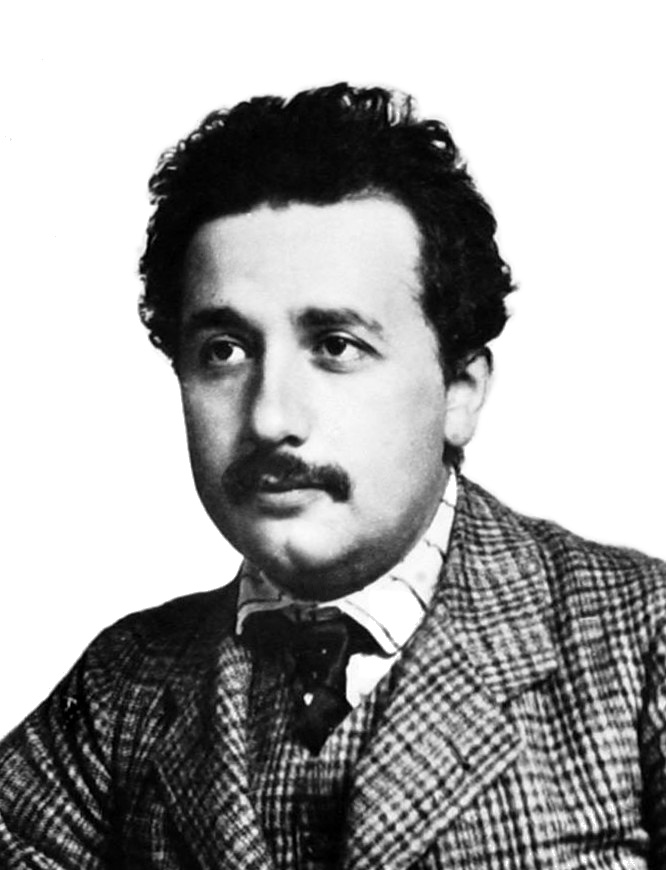
\includegraphics[width=1\linewidth]{images/Einstein_patentoffice.jpg}
	\caption[Photo of Albert Einstein]{From \href{https://commons.wikimedia.org/wiki/File:Einstein_patentoffice.jpg}{Wikimedia}: Albert Einstein around 1905, the year his "Annus Mirabilis papers" were published. These included Zur Elektrodynamik bewegter Körper, the paper founding special relativity.}
	\labfig{Einstein}
\end{marginfigure}
As we know, the Newton equations are not compatible with special relativity. Why? Because to compute accelerations we need to select a distinguish time axis and this is not compatible with the principle of \href{https://it.wikipedia.org/wiki/Relativit\%C3\%A0_ristretta}{special relativity}\footnote{In Albert Einstein's original treatment, the theory is based on two postulates:
\begin{enumerate}
    \item The laws of physics are invariant (that is, identical) in all inertial frames of reference (that is, frames of reference with no acceleration).
    \item The speed of light in vacuum is the same for all observers, regardless of the motion of the light source or observer.
\end{enumerate}
}. We have to replace the Newton equation with something else and the idea, due to Einstein itself, is based on the idea of proper time.
\subsection{Proper time}
We fix an inertial frame, or a Lorentzian chart\index{Lorentzian chart}, and we draw the \textbf{world line} of our particle.
\begin{marginfigure}
    \centering
	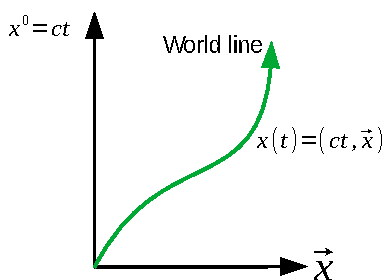
\includegraphics[width=1\linewidth]{images/World_line.pdf}
	\caption{Schematic representation of a world line.}
	\labfig{world_line}
\end{marginfigure}
Now we define the \textbf{proper time}, a sort of reparametrization of this path:  
\begin{equation}\labeq{tau}
\tau(t)=\int_{t_0}^t \sqrt{1-\frac{|\Vec{v}(t')|^2}{c^2}}\dd{t'}
\end{equation}
Physically, this is the time given by a clock moving with the system (comoving clock), synchronized at time $t=t_0$ with the official clock of the inertial frame.
\subsection{Tetra-velocity}
Once we are equipped with the proper time, we can define the \textbf{tetra-velocity}
\[
u^{\mu}(\tau):=\dv{x^{\mu}({\color{red}\tau})}{\color{red}\tau}
\]
What is its relation with the ordinary velocity? It is given by the chain rule:\marginnote{
\[
\norm{u}^2_g=\frac{c^2-v^2}{1-\frac{v^2}{c^2}^2}=\frac{1}{\frac{1}{c^2}}\frac{\cancel{c^2-v^2}}{\cancel{c^2-v^2}}=c^2
\]}
\begin{equation}\labeq{tetra-velocity}
u^{\mu}=\dv{x^{\mu}}{\tau}=\dv{x^{\mu}}{t}\dv{t}{\tau}=\dv{x^{\mu}}{t}\frac{1}{\textrm{d}\tau/\textrm{d} t}\overset{(\ref{eq:tau})}{=}\frac{1}{\sqrt{1-\frac{v(t)^2}{c^2}}}{\color{red}\dv{x^{\mu}(\tau(t))}{\underset{\mathclap{\tikz \node {$\uparrow$} node [below=1ex] {\footnotesize ordinary velocity };}}t}}\quad \Big|\Big| \quad \star
\end{equation}
What is remarkable is that the Lorentzian norm of the tetra-velocity is constant: $\rVert u \rVert^2_g=\langle u,u \rangle_g=c^2$. Suppose to have a particle at rest in the point $x_0$ which stays at rest forever: the world line will be equal to $(ct,\Vec{x_0})$, with tetra-velocity $(c,\Vec{0})$. This holds true for any other curve.\marginnote{The check of this relation is left as an exercise.}
\subsection{Tetra-acceleration}
We go on and we define the \textbf{tetra-acceleration}:
\[
a^{\mu}(\tau):=\dv{u^{\mu}(\tau)}{\color{red}\tau}
\]
The tetra-velocity has a peculiar geometric relation with the tetra-acceleration, in fact they are \textbf{Lorentz orthogonal}:\marginnote{Since the inner product is bilinear and continuous, we can apply the Leibniz property.}
\[
0=\dv{\tau}\langle u,u \rangle_g\underset{\mathclap{\tikz \node {$\uparrow$} node [below=1ex] {\footnotesize Leibniz };}}=\langle\dv{\tau}u,u\rangle_g+\langle u,\dv{\tau}u\rangle_g\underset{\mathclap{\tikz \node {$\uparrow$} node [below=1ex] {\footnotesize symmetric};}}=2\langle u,\dv{\tau}u\rangle_g=2\langle u,a \rangle_g
\]
it means that for any world line, i.e. any possible cinematic, ${\color{red}\langle u(\tau),a(\tau) \rangle_g=0}$, so geometrically it means they are orthogonal but with respect to the Lorentzian metric: ${\color{red}u(\tau)\perp_g a(\tau)}$.
\subsection{Relativistic version of Newton equation}
We are now ready to write the relativistic version of the Newton equation:\index{Tetra-force}
\[
\star \quad \Big|\Big| \quad m\dv{\tau}u^{\mu}(\tau)=\underbrace{f(x(\tau),u(\tau))}_{\textrm{tetra-force\marginnote{We sill have to understand the relation between the tetra-force and the ordinary force in three dimensional space.}}}
\]
Not every vector field on the Minkowski space is admissible as a tetra-force, because there is a constraint between the 0-component and the space-components.
The \textbf{orthogonality relation} ${\color{red}a\perp_g u}$ implies that also $f\perp_g u$, hence the 4-components of the tetra-force $f=(f^0,\vec{f})$ are \underline{\textbf{not}} \textbf{independent}:
\begin{equation}\labeq{non-ind-force}
0=\langle u,f \rangle_g\overset{\textrm{I.F.}}{=}cf^0-\vec{v}\cdot\vec{f}\quad \Rightarrow \quad \Big|\Big| \quad f^0(x,\underset{\mathclap{\tikz \node {$\uparrow$} node [below=1ex] {\footnotesize $(u^0,\vec{v})$};}}u)=\frac{1}{c}\vec{f}\cdot\vec{v}
\end{equation}
Explicitly, in an inertial frame, using \refeq{tetra-velocity}, RNE\sidenote{RNE$=$Relativistic Newton Equation} reads as follows:
\[
\begin{cases}
\dv{t}\frac{mc}{\sqrt{1-v^2/c^2}}=\sqrt{1-\frac{v^2}{c^2}}\,{\color{red}f^0}\quad \xRightarrow[]{(\ref{eq:non-ind-force})}\; \dv{t}\underbrace{\frac{mc^{\color{red}2}}{\sqrt{1-v^2/c^2}}}_{\mathclap{\text{relativistic kinetic energy\marginnote{$E_{\textrm{kin}}\simeq mc^2+\frac{1}{2}mv^2+\mathcal{O}(v/c)$ as $v/c\xrightarrow[]{}0$}}}}=\sqrt{1-\frac{v^2}{c^2}}{\color{red}\vec{f}\cdot\vec{v}}=\vec{F}\cdot\vec{v}\ \xleftarrow[]{}\text{power of $\vec{F}$} \\
\dv{t}\frac{m\vec{v}}{\sqrt{1-v^2/c^2}}=\sqrt{1-\frac{v^2}{c^2}}\vec{f}=:\vec{F}\ \xleftarrow[]{}\text{force field in the inertial frame}
\end{cases}
\]
Where the identification with the physical force field is suggested by experimental data and experience.
\section{Determination of tetra-force}
We now want to decide which kind of vector fields are admissible as a tetra-force, in particular which one corresponds to the usual Lorentz force of electrodynamics.
\begin{marginfigure}[-50mm]
	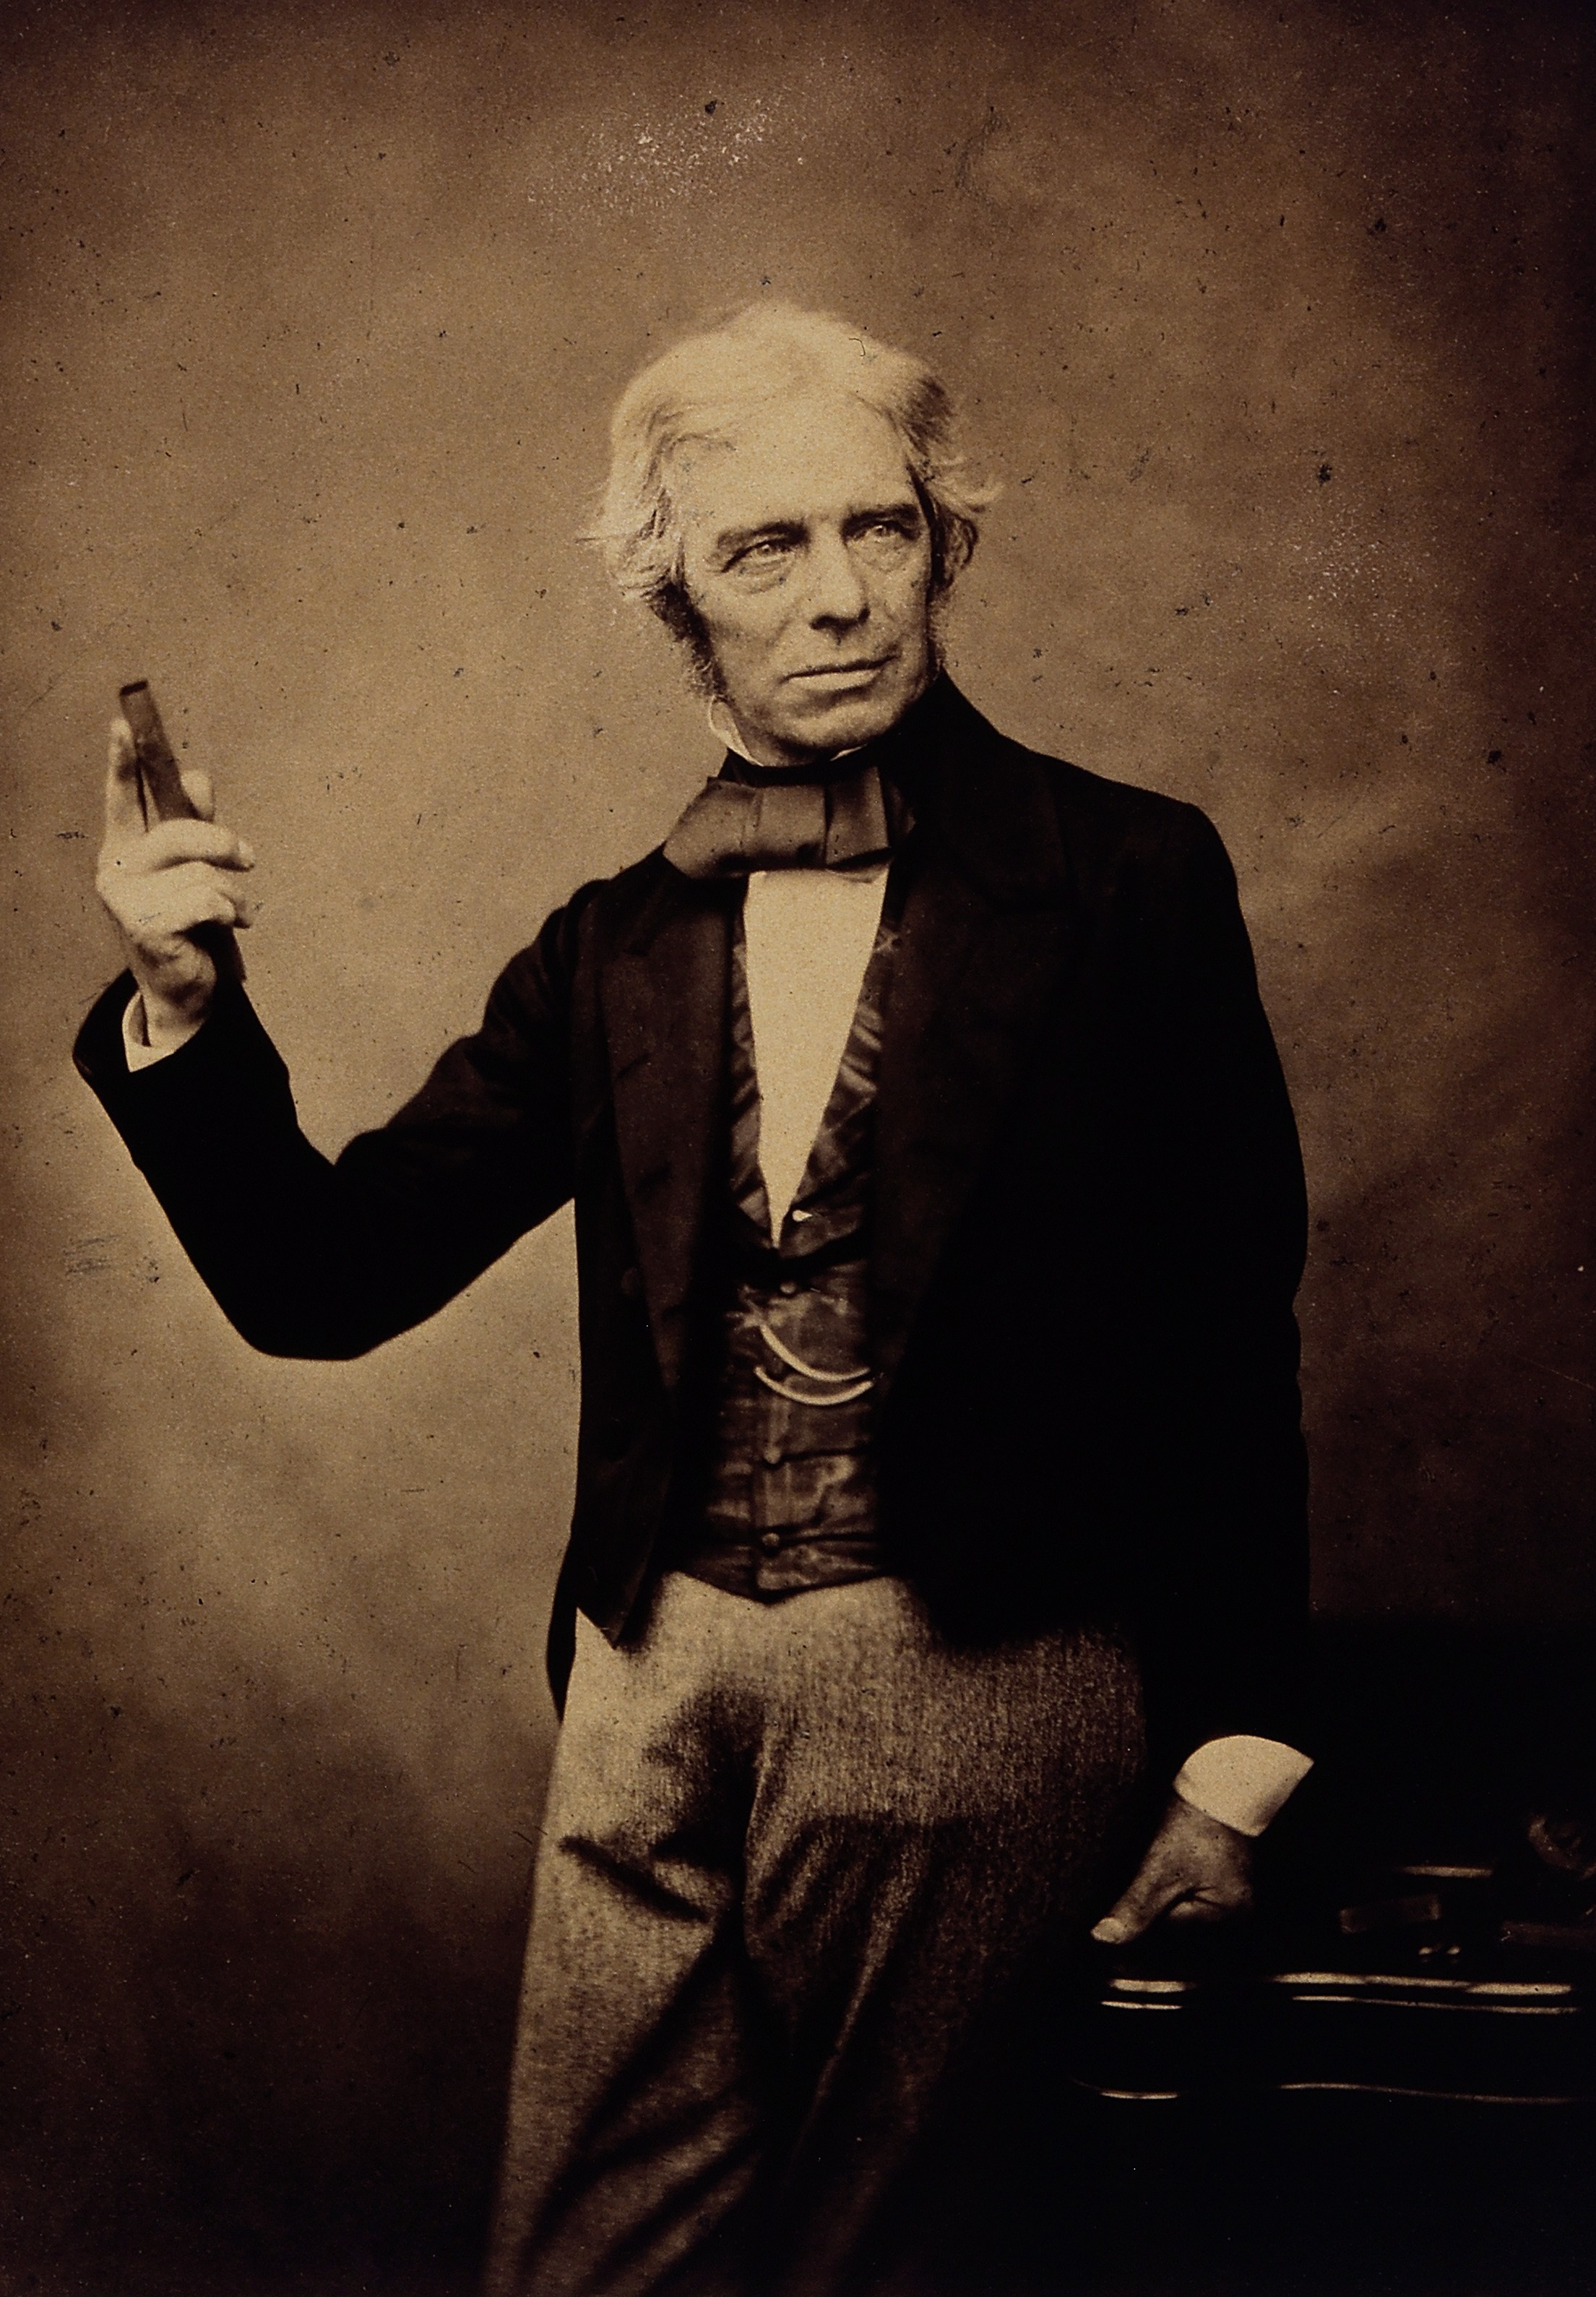
\includegraphics[width=1\linewidth]{images/MichaelFaraday.jpg}
	\caption[Michael Faraday. Photograph by Maull \& Polyblank. Iconographic Collections.]{From \href{https://commons.wikimedia.org/wiki/File:Michael\_Faraday.\_Photograph_by_Maull\_\%26\_Polyblank.\_Wellcome\_V0026348.jpg}{Wikimedia}: Michael Faraday. Photograph by Maull \& Polyblank. Iconographic Collections. Michael Faraday FRS was an English scientist who contributed to the study of electromagnetism and electrochemistry. His main discoveries include the principles underlying electromagnetic induction, diamagnetism and electrolysis. Albert Einstein kept a picture of Faraday on his study wall, alongside pictures of Arthur Schopenhauer and James Clerk Maxwell. Physicist Ernest Rutherford stated, "When we consider the magnitude and extent of his discoveries and their influence on the progress of science and of industry, there is no honour too great to pay to the memory of Faraday, one of the greatest scientific discoverers of all time." Faraday died at his house at Hampton Court on 25 August 1867, aged 75.}
	\labfig{Faraday}
\end{marginfigure}
\underline{Problem:} characterize tetra-forces such that $\langle f(x,u),u \rangle_g=0$.\\
$\triangleright$ We suppose that $f(x,u)$ \textbf{depends linearly on} $u$. From the physical viewpoint, we know that the Lorentz force is linear in the velocity and from the mathematical viewpoint, we remember that if a force field is more than linear in the velocity (i.e. quadratic, depends on $u^{3/2}$) then it is not compatible with the Lagrangian formalism. This means that
\[
f^{\mu}(x,u)=\sum_{\nu}\Tilde{F}_{\; \nu}^{\mu}(x)u^{\nu}
\]
$\triangleright$ We impose the constraint $\langle f(x,u),u \rangle_g=0$:
\[
\sum_{\sigma,\nu,\mu}u^{\sigma}\underbrace{g_{\sigma\mu}\Tilde{F}_{\nu}^{\;\mu}}_{\color{red}=:\Tilde{F}_{\sigma\nu}}u^{\nu}=\sum_{\sigma\nu}u^{\sigma}\Tilde{F}_{\sigma\nu}u^{\nu}=0 \quad \forall\; u\in T\mathbb{M}
\]
This implies that $\Tilde{F}_{\sigma\nu}$ is \textbf{anti-symmetric}: ${\color{red}\Tilde{F}_{\sigma\nu}=-\Tilde{F}_{\nu\sigma}}$. In fact:
\[
\begin{split}
\sum_{\color{red}\sigma<\nu}u^{\sigma}u^{\nu}\Tilde{F}_{\sigma\nu}(x) + \sum_{\color{red}\nu\leq\sigma}u^{\sigma}u^{\nu}\Tilde{F}_{\sigma\nu}(x)
&\overset{\mathclap{\tikz \node {$\downarrow$} node [above=1.25ex] {\footnotesize $\sigma'=\nu, \; \nu'=\sigma$};}}{=}\sum_{\color{red}\sigma<\nu}u^{\sigma}u^{\nu}\Tilde{F}_{\sigma\nu}(x) + \sum_{\color{red}\sigma'\leq\nu'}u^{\nu'}u^{\sigma'}\Tilde{F}_{\nu'\sigma'}(x)=\\
&=\sum_{\sigma<\nu}u^{\sigma}u^{\nu}\left[\Tilde{F}_{\sigma\nu}(x)+\Tilde{F}_{\nu\sigma}(x)\right]+\sum_\nu u^\nu u^\nu \Tilde{F}_{\nu\nu}=\\
&=0\qquad \forall\; u\in T\mathbb{M}
\end{split}
\]
\[
\Rightarrow\ {\color{red}\Tilde{F}_{\sigma\nu}(x)=-\Tilde{F}_{\nu\sigma}(x)}. \quad \textrm{(AS)}
\]
\underline{Conclusion:} An admissible tetra-force correspond to an \textbf{anti-symmetric, 2-covariant tensor field}, alias a \textbf{differential 2-form}
\[
\Tilde{\pazocal{F}}=\sum_{\mu<\nu}\Tilde{F}_{\mu\nu}(x)\;dx^{\mu}\wedge dx^{\nu}
\]
$\triangleright$ Now we add a piece of physical information: we know (experimentally) that in an inertial frame, the force field $\vec{F}$ is given by the \textbf{Lorentz force}:\marginnote{$q$ is the charge, $c$ is the speed of light.}
\begin{equation}\labeq{lorentz-force}
q\left[\vec{E}(x)+\frac{1}{c}\vec{v}\wedge\vec{B}(x)\right]^{\color{red}l}=\sqrt{1-\frac{v^2}{c^2}}\sum_{\nu=0}^3 \Tilde{F}_{\;\;\nu}^{{\color{red}\overset{\mathclap{\tikz \node {$\downarrow$} node [above=1.25ex] {\footnotesize space component};}}l}}(x)u^{\nu} \quad\text{for every } l\in\{1,2,3\} \quad (\star)
\end{equation}
$\triangleright$ As an exercise, one checks that \refeq{lorentz-force} holds true if and only if the covariant tensor $\Tilde{F}_{\mu\nu}(x)=\frac{q}{c}F_{\mu\nu}(x)$ is given by some explicit form:
\begin{equation}\labeq{Faraday-tensor}
F_{\mu\nu}(x)=\begin{pmatrix}
0 & -E_x & -E_y & -E_z \\
E_x & 0 & B_z & -B_y \\
E_y & -B_z & 0 & B_x \\
E_z & B_y & -B_x & 0
\end{pmatrix}\marginnote{The signs depend on all the other conventions, so maybe if you change book you will have something else.}
\end{equation}
This is the 2-tensor which represents the electromagnetic field, also called the \href{https://it.wikipedia.org/wiki/Tensore_elettromagnetico}{Faraday tensor}\sidenote{Although \href{https://en.wikipedia.org/wiki/Michael_Faraday}{Faraday} didn't know anything about 2-forms, since he started all the investigation about electromagnetism the tensor is called in this way (and also $F$ is the first letter of his surname). Other names are:\begin{itemize}
    \item tensore elettromagnetico;
    \item tensore del campo elettromagnetico;
    \item tensore dello sforzo del campo;
    \item bivettore di Maxwell.
\end{itemize}}\index{Faraday tensor}.\\
\underline{Conclusion:} The electromagnetic field is described in an inertial/Lorentzian frame by the \textbf{2-form} $\pazocal{F}\in\Omega^2(\mathbb{M})$.
\begin{equation}\labeq{Farday-tensor}
\star \quad \Big| \Big| \quad \Tilde{\pazocal{F}}=\sum_{\substack{\mu,\nu=0\\ \mu<\nu}}^3 {F}_{\mu\nu}(x)dx^{\mu}\wedge dx^{\nu}
\end{equation}
$\triangleright$ Now we have written the force field as a differential 2-form, which is intrinsic so it does not depend on the change of coordinates even if we leave the clean world of Lorentzian frames. By the invariance of 2-forms under general change of coordinates, the last formula \refeq{Farday-tensor} describes the electromagnetic field in \textbf{any system of coordinates (aka local chart)}.
\section[\href{https://it.wikipedia.org/wiki/James_Clerk_Maxwell}{Maxwell} equations]{\href{https://it.wikipedia.org/wiki/James_Clerk_Maxwell}{Maxwell} equations\sidenote{We write the equations using \href{https://it.wikipedia.org/wiki/Gauss_(unit\%C3\%A0_di_misura)}{Gauss units}.
We also denote with $\rho(x)$ the charge density, with $\vec{J}(x)$ the current density and with $x=(ct,\vec{x})$ a point in the spacetime.}}
\begin{subequations}
\labeq{Maxwell-eq}
\begin{align}
    \text{div}\vec{B} &=0 & \text{rot}\vec{E} &=-\frac{1}{c}\frac{\partial\vec{B}}{\partial t} & \small{\text{homogeneous}}\labeq{Homo-Maxwell}\\
    \text{div}\vec{E} &=4\pi\rho &
    \text{rot}\vec{B} &=\frac{1}{c}\frac{\partial\vec{E}}{\partial t}+\frac{4\pi}{c}\vec{J} & \small{\text{inhomogeneous}}\\
    & \hspace{-1.85em}\small{\text{constraints}} & & \hspace{-1.75em}\small{\text{dynamical equations}}\nonumber
\end{align}
\end{subequations}
\begin{marginfigure}[-10mm]
	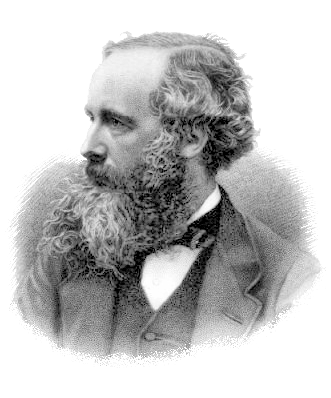
\includegraphics[width=1\linewidth]{images/James_Clerk_Maxwell.png}
	\caption[Photo of Maxwell]{From \href{https://commons.wikimedia.org/wiki/File:James_Clerk_Maxwell.png}{Wikimedia}: James Clerk Maxwell.}
	\labfig{Maxwell}
\end{marginfigure}The \textbf{homogeneous} equations are linear partial differential equations with no external terms, i.e. no sources, while the \textbf{inhomogeneous} equations instead contain the sources and they give us information about the relation with the distribution of charge and currents in the system. The homogeneous equation can also be written as $\dd\beta=0$ and $\dd\eta=0$. Sometimes, it is also convenient to read them by columns: the \textbf{dynamical equations} tell us how the fields evolve and the \textbf{constraints} state which conditions the vector fields have to satisfy at every time. We are going to proceed by row. Suppose we are in the stationary case, i.e. no time derivative, and let's look at the \textbf{homogeneous} equation: they are both \textbf{conditions of closureness} of differential forms.
\[
\dd{\beta}=0 \;\text{ with } \beta=\sum_{\substack{i,j=1\\i<j}}^3\mathbb{B}(x)_{ij}dx^i\wedge dx^j \quad \dd{\eta}=0 \;\text{ with } \eta=\sum_{i=1}^3 E_i(x)dx^i
\]
$\beta$ is builded up by the $3\times3$ part of the Faraday tensor while $\eta$ is builded up with the rows\marginnote{Or the columns, it is up to a sign and it depends on the convention used.} of the Faraday tensor.
\begin{proposition}
The \textbf{homogeneous Maxwell equations}\index{Homogeneous Maxwell equations}, which are written in an inertial frame, are equivalent to the intrinsic equation \begin{equation}\labeq{intrinsic-eq-2}
\dd{\pazocal{F}}=0
\end{equation}
where $\pazocal{F}=\sum F_{\mu\nu}(x)dx^{\mu}\wedge dx^{\nu}$ is the Faraday tensor of \refeq{Faraday-tensor}. In components:\marginnote{A trick to remember it the indices is to cycle them always in the same direction! Also, some people refer to it as equation Bianchi identity but we are not sure this is historically accurate.}
\begin{equation}\labeq{intrinsic-eq-3}
\partial_{\rho}F_{\mu\nu}+\partial_{\nu}F_{\rho\mu}+\partial_{\mu}F_{\nu\rho}=0
\end{equation}
where $\partial_{\rho}=\frac{\partial}{\partial x^{\rho}}$ and $(x^0,x^1,x^2,x^3)$ are local coordinates, not necessarily Lorentzian coordinates.
\end{proposition}
\begin{proof} We will proof \((\ref{eq:intrinsic-eq-2}) \Leftrightarrow (\ref{eq:intrinsic-eq-3})\)
\WithArrowsOptions{displaystyle}
\[
\begin{WithArrows}
\dd{\pazocal{F}}&\overset{\mathclap{\tikz \node {$\downarrow$} node [above=1.25ex] {\footnotesize by definition};}}{=}\sum_{\mu<\nu}(\dd{F}_{\mu\nu}(x))\wedge dx^{\mu}\wedge dx^{\nu}=\\
&=\sum_{\mu<\nu}\sum_{\lambda}\frac{\partial F_{\mu\nu}}{\partial x^{\lambda}}(x)\;dx^{\lambda}\wedge dx^{\mu}\wedge dx^{\nu}=\marginnote{The indices $\mu,\nu,\lambda$ are not well ordered, so we regroup them. $\lambda$ cannot be equal to $\mu$ or $\nu$ otherwise we will have zero. Each permutation brings a minus sign.}\\
&=\sum_{{\color{red}\lambda}<\mu<\nu}\frac{\partial F_{\mu\nu}}{\partial x^{\lambda}}(x)\;dx^{\lambda}\wedge dx^{\mu}\wedge dx^{\nu}+\\
&\quad+{\color{red}(-1)}\sum_{\mu<{\color{red}\lambda}<\nu}\frac{\partial F_{\mu\nu}}{\partial x^{\lambda}}(x)\;dx^{\mu}\wedge {\color{red}dx^{\lambda}}\wedge dx^{\nu}+\\
&\qquad+{\color{red}(-1)^2}\sum_{\mu<\nu<{\color{red}\lambda}}\frac{\partial F_{\mu\nu}}{\partial x^{\lambda}}(x)\;dx^{\mu}\wedge dx^{\nu}\wedge {\color{red}dx^{\lambda}}=\Arrow{We re-label the indices.}\\
&=\sum_{{\color{red}\lambda<\mu<\nu}}\left(\frac{\partial F_{\mu\nu}}{\partial x^{\lambda}}{\color{red}-}\frac{\partial F_{\lambda\nu}}{\partial x^{\mu}}+\frac{\partial F_{\lambda\mu}}{\partial x^{\nu}}\right)dx^{\lambda}\wedge dx^{\mu}\wedge dx^{\nu}=\Arrow{We exchange the indices $\lambda$ and $\nu$\\in the second term to produce a minus.}\\
&=\sum_{\lambda<\mu<\nu}\left(\frac{\partial F_{\mu\nu}}{\partial x^{\lambda}}{\color{red}+}\frac{\partial F_{\nu\lambda}}{\partial x^{\mu}}+\frac{\partial F_{\lambda\mu}}{\partial x^{\nu}}\right)dx^{\lambda}\wedge dx^{\mu}\wedge dx^{\nu}
\end{WithArrows}
\]
Which gives (\ref{eq:intrinsic-eq-3}).
\end{proof}
Then there is the equivalence of \((\ref{eq:Homo-Maxwell}) \Leftrightarrow (\ref{eq:intrinsic-eq-2}) \) (or $(\ref{eq:intrinsic-eq-3})$), but this is left as an exercise.
We have now a powerful tool, which is the theory of differential forms, which allows us to prove in one line the existence of electromagnetic potential:
\begin{proposition}
There exists a 1-form $\alpha=\sum_{\mu=0}^3A_{\mu}(x)dx^{\mu}$ such that the external differential of alpha is the Farady tensor {\color{red}$\dd{\alpha}=\pazocal{F}$} i.e.
\[
{\color{red}F_{\mu\nu}(x)=\partial_{\mu}A_{\nu}(x)-\partial_{\nu}A_{\mu}(x)}.
\]
\end{proposition}
\begin{proof}
Observe that $\mathbb{M}\cong\mathbb{R}^4$ is contractible, which means it can be continuously deformed to a point. By the converse of the Poincaré \reflemma{Converse-to-Poincaré-lemma}, since {\color{red}$\dd{\pazocal{F}}=0$ (Maxwell equations)}, then there $\exists\;\alpha\in\Omega^1(\mathbb{M})$ such that $\dd{\alpha}=\pazocal{F}$.
\end{proof}
We explicitly compute it now: the covariant components of the potential are\marginnote{The signs are correct, because there are the covariant components.}
\[
A_0=V \quad\qquad A_1=-A_x \ ,\quad A_2=-A_y \ ,\quad A_3=-A_z
\]
If we want the contravariant components, the corresponding \textbf{vector field} is {\color{red}$A^{\mu}=g^{\mu\nu}A_{\nu}$} where $\left(g^{\mu\nu}\right)=(G^{-1})^{\mu\nu}$\marginnote{If the ordinary metric is $\left(g_{\mu\nu}\right)=G$, then when we go to the indices upstairs, we should take the inverse matrix. The Lorentzian metric is special because $G=G^{-1}$}:
\[
A^0=V \quad\qquad A^1=A_x \ ,\quad A^2=A_y \ ,\quad A^3=A_z
\]
What is the message to take home? Any tetra-form has a relation between the 0-component and the spatial components and to be admissible it has to be given by a 2-covariant anti-symmetric tensor field which is a differential 2-form. If we insert a bit of physical information we get the Faraday tensor. Once we write it as a differential form, this holds true in any coordinate system.\\
How about the \textbf{inhomogeneous} Maxwell equation? Unlike the homogeneous ones\sidenote{Which are very geometrical.}, they are partially geometrical but that is because they involve the \underline{sources} and there is no reason why they should be geometrical. The sources are completely described by a contravariant vector called the \textbf{tetra-current}:
\[
\pqty{j^{\mu}(x)}=\left(c\rho(t,\vec{x}),\vec{j}(t,\vec{x})\right)
\]
The \underline{\textbf{continuity equation}}, which expresses the fact that the charge is locally conserved, in this formalism it can be written down as:
\[
\sum_{\mu=0}^3\partial_{\mu}j^{\mu}(x)=0
\]
We want \textbf{I order PDEs\sidenote{PDE = Partial Differential Equation}}\index{PDE} which involve a datum $j^{\mu}(x)$, which is contravariant, and either $F_{\mu\nu}$ or one of its "relatives" ($F_{\mu}^{\;\;\nu},F^{\mu\nu},\dots$). There are not many possibilities to satisfy this:
\[
\sum_{\nu=0}^3\partial_{\nu}F^{\mu\nu}=\frac{4\pi}{c}j^{\mu} \qquad \Big| \Big| \quad \small{\text{Inhomogeneous Maxwell equations}}
\]
where $F^{\mu\nu}=g^{\mu\sigma}g^{\nu\rho}F_{\sigma\rho}$. If we consider the \textbf{Minkowski metric} the corresponding matrix is diagonal:\marginnote{IF = Inertial Frame}
\[
g^{\mu\nu}=g^{\mu\mu}\delta^{\mu\nu} \qquad F^{\mu\nu}=g^{\mu\nu}g^{\nu\nu}F_{\mu\nu} \quad (\textrm{in $\mathbb{M}$, IF})
\]
The Faraday tensor now becomes:
\[
F^{\mu\nu}=\begin{pmatrix}
0 & E_x & E_y & E_z \\
-E_x & 0 & B_z & -B_y \\
-E_y & -B_z & 0 & B_x \\
-E_z & B_y & -B_x & 0
\end{pmatrix}
\]
We notice that for $\text{ with } \mu,\nu\in\{1,2,3\}$ the components are unchanged.
\end{document}